\documentclass[
]{jss}

%% recommended packages
\usepackage{orcidlink,thumbpdf,lmodern}

\usepackage[utf8]{inputenc}

\author{
Hanne I. Oberman\\Methodology and Statistics\\
Utrecht University \And Johanna Muñoz\\Julius Center for Health Sciences
and Primary Care,\\
University Medical Center Utrecht, Utrecht University,\\
Utrecht, The Netherlands \AND Thomas P. A. Debray\\Julius Center
for Health Sciences and Primary Care,\\
University Medical Center Utrecht, Utrecht University,\\
Utrecht, The Netherlands \And Gerko Vink\\Methodology and Statistics\\
Utrecht University \AND Valentijn M. T. de Jong\\Julius Center for
Health Sciences and Primary Care,\\
University Medical Center Utrecht, Utrecht University,\\
Utrecht, The Netherlands\\
Data Analytics and Methods Task Force,\\
European Medicines Agency,\\
Amsterdam, The Netherlands
}
\title{Imputation of Incomplete Multilevel Data with \pkg{mice}}

\Plainauthor{Hanne I. Oberman, Johanna Muñoz, Thomas P. A. Debray, Gerko
Vink, Valentijn M. T. de Jong}
\Plaintitle{Imputation of Incomplete Multilevel Data with mice}
\Shorttitle{Multilevel \pkg{mice}}


\Abstract{
This tutorial illustrates the imputation of incomplete multilevel data
with the \proglang{R} packackage \pkg{mice}. Our scope is only simple
multilevel models, to show how imputation can yield less biased
estimates from incomplete clustered data. More complex models can be
accomodated, but are outside the scope of this paper.
}

\Keywords{missing
data, multilevel, clustering, \pkg{mice}, \proglang{R}}
\Plainkeywords{missing data, multilevel, clustering, mice, R}

%% publication information
%% \Volume{50}
%% \Issue{9}
%% \Month{June}
%% \Year{2012}
%% \Submitdate{}
%% \Acceptdate{2012-06-04}

\Address{
    Hanne I. Oberman\\
    Methodology and Statistics\\
Utrecht University\\
    Padualaan 14\\
3584 CH Utrecht\\
  E-mail: \email{h.i.oberman@uu.nl}\\
  URL: \url{https://hanneoberman.github.io/}\\~\\
          }


% tightlist command for lists without linebreak
\providecommand{\tightlist}{%
  \setlength{\itemsep}{0pt}\setlength{\parskip}{0pt}}

% From pandoc table feature
\usepackage{longtable,booktabs,array}
\usepackage{calc} % for calculating minipage widths
% Correct order of tables after \paragraph or \subparagraph
\usepackage{etoolbox}
\makeatletter
\patchcmd\longtable{\par}{\if@noskipsec\mbox{}\fi\par}{}{}
\makeatother
% Allow footnotes in longtable head/foot
\IfFileExists{footnotehyper.sty}{\usepackage{footnotehyper}}{\usepackage{footnote}}
\makesavenoteenv{longtable}


\usepackage{graphicx}
\usepackage{mathtools}
\usepackage{ulem}

\usepackage{amsmath}

\begin{document}



\hypertarget{introduction}{%
\section{Introduction}\label{introduction}}

Many datasets include individuals that are clustered together, for
example in geographic regions, or even different studies. In the
simplest case, individuals (e.g., students) are nested within a single
cluster (e.g., school classes). More complex clustered structures may
occur when there are multiple hierarchical levels (e.g., students in
different schools or patients within hospitals within regions across
countries), or when the clustering is non-nested (e.g., electronic
health record data from diverse settings and populations within large
databases). With clustered data we generally assume that individuals
from the same cluster tend to be more similar than individuals from
other clusters. In statistical terms, this implies that observations
from the same cluster are not independent and may in fact be correlated.
If this correlation is left unaddressed, estimates of \emph{p} values,
confidence intervals even model parameters are prone to bias
\citep{loca01}. Statistical methods for clustered data typically adopt
hierarchical models that explicitly describe the grouping of
observations. These models are also known as `multilevel models',
`hierarchical models', `mixed effect models', `random effect models',
and in the context of time-to-event data as `frailty models'. Table
\ref{tab:clus} provides an overview of some key concepts in multilevel
modeling.

\begin{CodeChunk}
\begin{table}

\caption{\label{tab:clus}Concepts in multilevel methods}
\centering
\begin{tabular}[t]{>{\raggedright\arraybackslash}p{3cm}>{\raggedright\arraybackslash}p{12cm}}
\toprule
Concept & Details\\
\midrule
Sample unit & Units of the population from which measurements are taken in a sample.\\
Hierarchical levels & Data are grouped into clusters at different levels, observations belonging to the same cluster are expected to share certain characteristics.\\
Fixed effect & Effects that are constant across all sample units, e.g. something that researchers control for and can repeat, such as the administration of a drug.\\
Random effect & Effects that are a source of random variation in the data, and whose levels are not fully sampled. e.g. individuals are drawn from a population of hospitals, here it is not possible to sample all hospitals but drug effects could vary between hospitals.\\
Mixed effect & Includes fixed and random effects, e.g. the fixed effect would be the treatment effect of a drug and the random effect would be the ID of the hospital where the patient is treated. Multilevel models typically accommodate for variability by including a separate group mean for each cluster e.g random intercept on hospitals. In addition to random intercepts, multilevel models can also include random coefficients and heterogeneous residual error variances across clusters (see e.g. @gelm06, @hox17 and @jong21).\\
\addlinespace
ICC & The variability due to clustering is often measured by means of the intraclass coefficient (ICC). The ICC can be seen as the percentage
of variance that can be attributed to the cluster-level, where a high ICC would indicate that a lot of variability is due to the cluster structure.\\
Stratified intercept & \\
\bottomrule
\end{tabular}
\end{table}

\end{CodeChunk}

\hypertarget{missingness-in-multilevel-data}{%
\subsection{Missingness in multilevel
data}\label{missingness-in-multilevel-data}}

As with any other dataset, clustered datasets may be impacted by
missingness in much the same way. Several strategies can be used to
handle missing data, including complete case analysis and imputation. We
focus on the latter approach and discuss statistical methods for
replacing the missing data with one or more plausible values. Imputation
separates the missing data problem from the analysis and the completed
data can be analyzed as if it were completely observed. It is generally
recommended to impute the missing values more than once to preserve
uncertainty due to missingness and to allow for valid inferences (c.f.
Rubin 1976).

With incomplete clustered datasets we can distinguish between two types
of missing data: sporadic missingness and systematic missingness
\citep{resc13}. Sporadic missingness arises when variables are missing
for some but not all of the units in a cluster \citep{buur18, jola18}.
For example, it is possible that test results are missing for several
students in one or more classes. When all observations are missing
within one or more clusters, data are said to be systematically missing.

\begin{CodeChunk}
\begin{figure}

{\centering 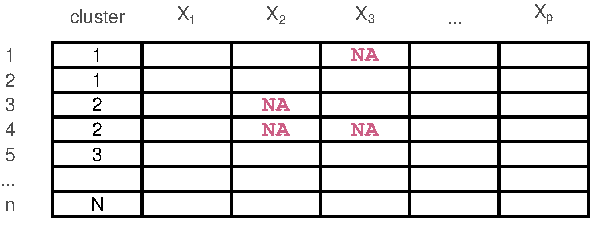
\includegraphics{Imputation_of_Incomplete_Multilevel_Data_files/figure-latex/patterns-1} 

}

\caption[Sporadic missingness in multilevel data]{Sporadic missingness in multilevel data}\label{fig:patterns}
\end{figure}
\end{CodeChunk}

Imputation of missing data requires consideration of the mechanism
behind the missingness. Rubin proposed to distinguish between data that
are missing completely at random (MCAR), data that are missing at random
(MAR) and data that are missing not at random (MNAR; see Table
\ref{tab:miss}). For each of these three missingness generating
mechanisms, different imputation strategies are warranted
(\citet{yuce08} and \citet{hox15}). We here consider the general case
that data are MAR, and expand on certain MNAR situations.

Table 2: Concepts in missing data methods

\begin{longtable}[]{@{}
  >{\raggedright\arraybackslash}p{(\columnwidth - 2\tabcolsep) * \real{0.1739}}
  >{\raggedright\arraybackslash}p{(\columnwidth - 2\tabcolsep) * \real{0.8261}}@{}}
\toprule\noalign{}
\begin{minipage}[b]{\linewidth}\raggedright
\textbf{Concept}
\end{minipage} & \begin{minipage}[b]{\linewidth}\raggedright
\textbf{Details}
\end{minipage} \\
\midrule\noalign{}
\endhead
\bottomrule\noalign{}
\endlastfoot
MCAR & Missing Completely At Random, where the probability to be missing
is equal \\
& across all data entries \\
MAR & Missing At Random, where the probability to be missing depends on
observed \\
& information \\
MNAR & Missing Not At Random (MNAR), where the probability to be
missing \\
& depends on unrecorded information, making the missingness
non-ignorable \\
& \citep{rubi76, meng94}. \\
& \\
\end{longtable}

\hypertarget{aim-of-this-paper}{%
\subsection{Aim of this paper}\label{aim-of-this-paper}}

This papers serves as a tutorial for imputing incomplete multilevel data
with \pkg{mice} in \proglang{R}. \pkg{mice} has become the de-facto
standard for imputation by chained equations, which iteratively solves
the missingness on a variable-by-variable basis. \pkg{mice} is known to
yield valid inferences under many different missing data circumstances
\citep{buur18}.

We provide practical guidelines and code snippets for different missing
data situations, including non-ignorable mechanisms. For reasons of
brevity, we focus on multilevel imputation by chained equations with
\pkg{mice} exclusively; other imputation methods and packages \citep[see
e.g.][ and \citet{grun18}]{audi18} are outside the scope of this
tutorial. Assumed knowledge includes basic familiarity with the
\pkg{lme4} notation for multilevel models (see Table \ref{tab:mod}).

We illustrate imputation of incomplete multilevel data using three case
studies:

\begin{itemize}
\tightlist
\item
  \texttt{popmis} from the \pkg{mice} package \citep[simulated data on
  perceived popularity, \(n = 2,000\) pupils across \(N = 100\) schools
  with data that are MAR,][]{mice};
\item
  \texttt{impact} from the \pkg{metamisc} package \citep[empirical data
  on traumatic brain injuries, \(n = 11,022\) patients across \(N = 15\)
  studies with data that are MAR,][]{metamisc};
\item
  \texttt{obesity} from the \pkg{micemd} package {[}simulated data on
  obesity, \(n = 2,111\) patients across \(N = 5\) regions with data
  that are MNAR{]}.
\end{itemize}

For each of these datasets, we discuss the nature of the missingness,
choose one or more imputation models and evaluate the imputed data, but
we will also highlight one specific aspect of the imputation workflow.

This tutorial is dedicated to readers who are unfamiliar with multiple
imputation. More experienced readers can skip the introduction (case
study 1) and directly head to practical applications of multilevel
imputation under MAR conditions (case study 2) or under MNAR conditions
(case study 3).

\hypertarget{setup}{%
\subsection{Setup}\label{setup}}

Install non-CRAN packages if necessary:

\begin{CodeChunk}
\begin{CodeInput}
R> devtools::install_github("amices/ggmice")
\end{CodeInput}
\end{CodeChunk}

Set up the R environment and load the necessary packages:

\begin{CodeChunk}
\begin{CodeInput}
R> set.seed(2022)        # for reproducibility
R> library(mice)         # for imputation
R> library(miceadds)     # for additional imputation routines
R> library(ggmice)       # for incomplete/imputed data visualization
R> library(ggplot2)      # for visualization
R> library(dplyr)        # for data wrangling
R> library(lme4)         # for multilevel modeling
R> library(mitml)        # for multilevel parameter pooling
R> library(micemd)  # for imputation cf. heckman models
R> library(metamisc)     # for case study data
\end{CodeInput}
\end{CodeChunk}

\hypertarget{case-study-i-popularity-data}{%
\section{Case study I: popularity
data}\label{case-study-i-popularity-data}}

In this section we will go over the different steps involved with
imputing incomplete multilevel data with the R package mice. We consider
the simulated \texttt{popmis} dataset, which included pupils
(\(n = 2000\)) clustered within schools (\(N = 100\)). The following
variables are of primary interest:

\begin{itemize}
\tightlist
\item
  \texttt{school}, school identification number (clustering variable);
\item
  \texttt{popular}, pupil popularity (self-rating between 0 and 10;
  unit-level);
\item
  \texttt{sex}, pupil sex (0=boy, 1=girl; unit-level);
\item
  \texttt{texp}, teacher experience (in years; cluster-level).
\end{itemize}

The research objective of the \texttt{popmis} dataset is to predict the
pupils' popularity based on their gender and the experience of the
teacher. The analysis model corresponding to this dataset is multilevel
regression with random intercepts, random slopes and a cross-level
interaction. The outcome variable is \texttt{popular}, which is
predicted from the unit-level variable \texttt{sex} and the
cluster-level variable \texttt{texp}:

\begin{CodeChunk}
\begin{CodeInput}
R> mod <- popular ~ 1 + sex + (1 | school)
\end{CodeInput}
\end{CodeChunk}

Load the data into the environment and select the relevant variables:

\begin{CodeChunk}
\begin{CodeInput}
R> popmis <- popmis[, c("school", "popular", "sex")] 
\end{CodeInput}
\end{CodeChunk}

First we plot the pattern of missing data within categories of the
relevant variables. Plot the missing data pattern:

\begin{CodeChunk}
\begin{CodeInput}
R> plot_pattern(popmis)
\end{CodeInput}
\begin{figure}

{\centering 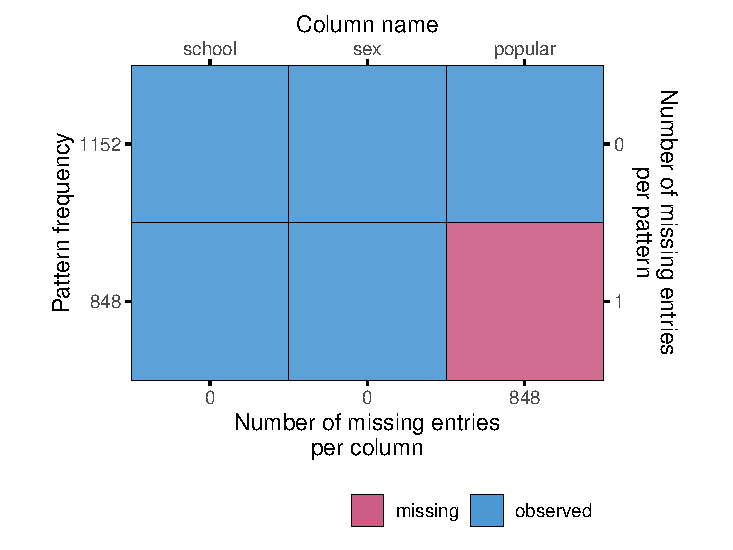
\includegraphics{Imputation_of_Incomplete_Multilevel_Data_files/figure-latex/pop_pat-1} 

}

\caption[Missing data pattern in the popularity data]{Missing data pattern in the popularity data}\label{fig:pop_pat}
\end{figure}
\end{CodeChunk}

The missingness is univariate and sporadic, which is illustrated in the
missing data pattern in Figure \ref{fig:pop_pat}.

To develop the best imputation model for the incomplete variable
\texttt{popular}, we need to know whether the observed values of
\texttt{popular} are related to observed values of other variables. Plot
the pair-wise complete correlations in the incomplete data:

\begin{CodeChunk}
\begin{CodeInput}
R> plot_corr(popmis)
\end{CodeInput}


\begin{center}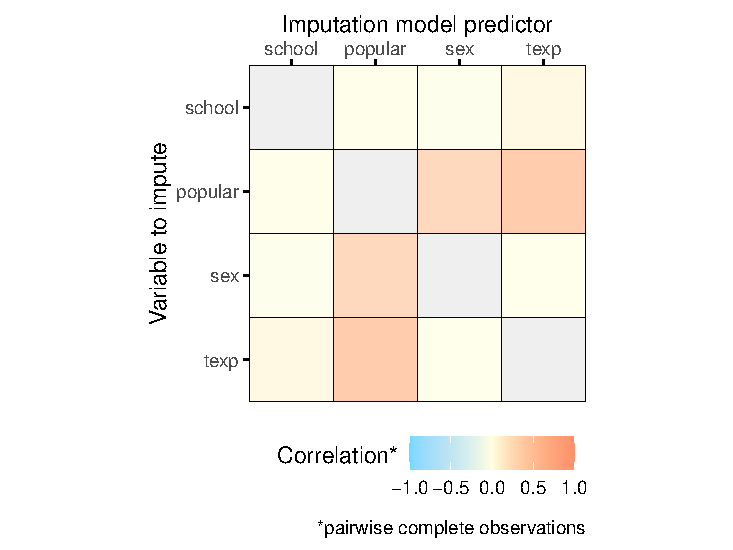
\includegraphics{Imputation_of_Incomplete_Multilevel_Data_files/figure-latex/pop-corr-1} \end{center}

\end{CodeChunk}

This shows us that \texttt{sex} may be a useful imputation model
predictor. Moreover, the missingness in \texttt{popular} may depend on
the observed values of other variables.

\begin{CodeChunk}
\begin{CodeInput}
R> # ggmice(popmis, aes(sex)) +
R> #   geom_histogram(fill = "white") +
R> #   facet_grid(. ~ is.na(popular), scales = "free", labeller = label_both)
R> 
R> ggplot(popmis, aes(y = popular, group = sex)) +
+   geom_boxplot() + 
+   theme_classic()
\end{CodeInput}


\begin{center}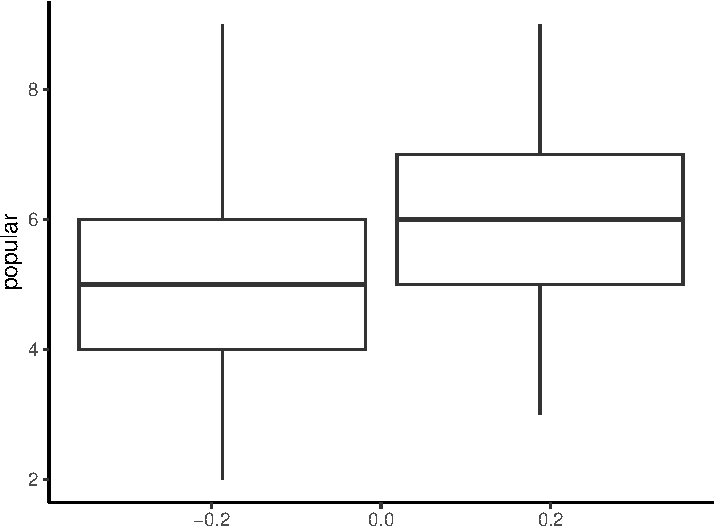
\includegraphics{Imputation_of_Incomplete_Multilevel_Data_files/figure-latex/pop-hist-1} \end{center}

\end{CodeChunk}

\hypertarget{imputation-ignoring-the-cluster-variable-not-recommended}{%
\subsubsection{Imputation ignoring the cluster variable (not
recommended)}\label{imputation-ignoring-the-cluster-variable-not-recommended}}

The first imputation model that we'll use is likely to be invalid. We do
\emph{not} use the cluster identifier \texttt{school} as imputation
model predictor. With this model, we ignore the multilevel structure of
the data, despite the high ICC. This assumes exchangeability between
units. We include it purely to illustrate the effects of ignoring the
clustering in our imputation effort.

Create a methods vector and predictor matrix for \texttt{popular}, and
make sure \texttt{school} is not included as predictor:

\begin{CodeChunk}
\begin{CodeInput}
R> meth <- make.method(popmis) # methods vector
R> pred <- quickpred(popmis)   # predictor matrix
R> plot_pred(pred)
\end{CodeInput}


\begin{center}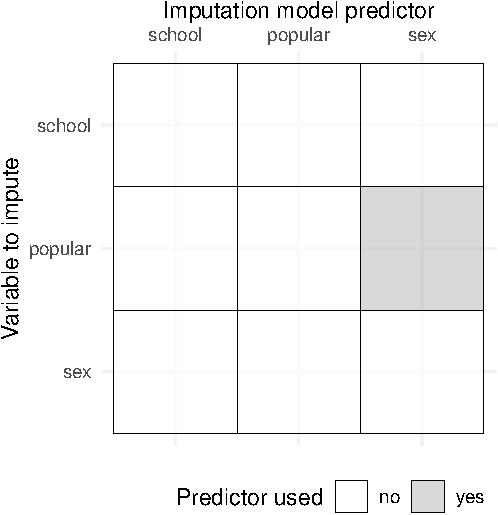
\includegraphics{Imputation_of_Incomplete_Multilevel_Data_files/figure-latex/pop-ignored-pred-1} \end{center}

\end{CodeChunk}

Impute the data, ignoring the cluster structure:

\begin{CodeChunk}
\begin{CodeInput}
R> imp <- mice(popmis, pred = pred, print = FALSE)
\end{CodeInput}
\end{CodeChunk}

Analyze the imputations:

\begin{CodeChunk}
\begin{CodeInput}
R> fit <- with(imp, 
+             lmer(popular ~ 1 + sex  + (1 | school))) 
\end{CodeInput}
\end{CodeChunk}

Print the estimates:

\begin{CodeChunk}
\begin{CodeInput}
R> testEstimates(as.mitml.result(fit), extra.pars = TRUE)
\end{CodeInput}
\begin{CodeOutput}

Call:

testEstimates(model = as.mitml.result(fit), extra.pars = TRUE)

Final parameter estimates and inferences obtained from 5 imputed data sets.

             Estimate Std.Error   t.value        df   P(>|t|)       RIV       FMI 
(Intercept)     5.012     0.295    16.994     4.362     0.000    22.587     0.969 
sex             0.695     0.251     2.768     4.287     0.047    28.390     0.975 

                            Estimate 
Intercept~~Intercept|school    0.266 
Residual~~Residual             1.035 
ICC|school                     0.208 

Unadjusted hypothesis test as appropriate in larger samples.
\end{CodeOutput}
\end{CodeChunk}

\hypertarget{imputation-with-the-cluster-variable-as-predictor-not-recommended}{%
\subsubsection{Imputation with the cluster variable as predictor (not
recommended)}\label{imputation-with-the-cluster-variable-as-predictor-not-recommended}}

We'll now use \texttt{school} as a predictor to impute all other
variables. This is still not recommended practice, since it only works
under certain circumstances and results may be biased
\citep{drec15, ende16}. But at least, it includes some multilevel
aspect. This method is also called `fixed cluster imputation', and uses
N-1 indicator variables representing allocation of N clusters as a fixed
factor in the model \citep{reit06, ende16}. Colloquially, this is
`multilevel imputation for dummies'.

\begin{CodeChunk}
\begin{CodeInput}
R> # adjust the predictor matrix
R> pred["popular", "school"] <- 1 
R> plot_pred(pred)
\end{CodeInput}


\begin{center}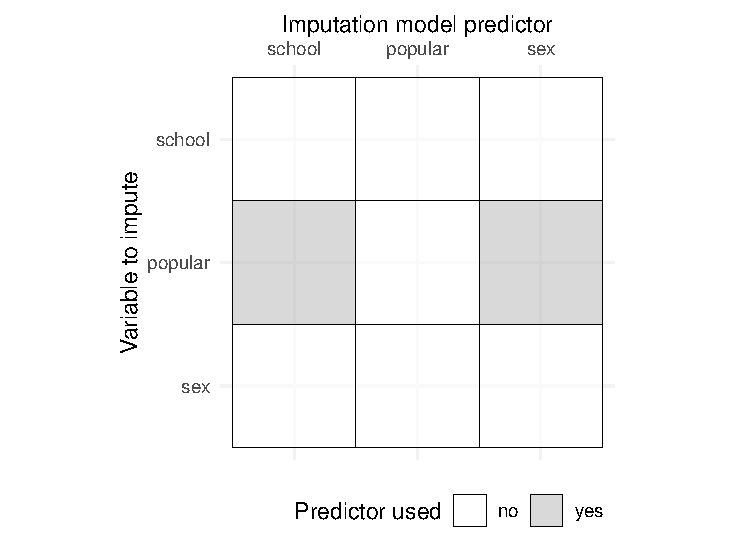
\includegraphics{Imputation_of_Incomplete_Multilevel_Data_files/figure-latex/pop_predictor-1} \end{center}

\begin{CodeInput}
R> # impute the data, cluster as predictor
R> imp <- mice(popmis, pred = pred, print = FALSE)
\end{CodeInput}
\end{CodeChunk}

Analyze the imputations:

\begin{CodeChunk}
\begin{CodeInput}
R> fit <- with(imp, 
+             lmer(popular ~ 1 + sex + (1 | school))) 
\end{CodeInput}
\end{CodeChunk}

Print the estimates:

\begin{CodeChunk}
\begin{CodeInput}
R> testEstimates(as.mitml.result(fit), extra.pars = TRUE)
\end{CodeInput}
\begin{CodeOutput}

Call:

testEstimates(model = as.mitml.result(fit), extra.pars = TRUE)

Final parameter estimates and inferences obtained from 5 imputed data sets.

             Estimate Std.Error   t.value        df   P(>|t|)       RIV       FMI 
(Intercept)     4.915     0.217    22.642     4.926     0.000     9.110     0.926 
sex             0.975     0.283     3.444     4.250     0.024    32.504     0.978 

                            Estimate 
Intercept~~Intercept|school    0.351 
Residual~~Residual             1.153 
ICC|school                     0.233 

Unadjusted hypothesis test as appropriate in larger samples.
\end{CodeOutput}
\end{CodeChunk}

\hypertarget{imputation-with-multilevel-model}{%
\subsubsection{Imputation with multilevel
model}\label{imputation-with-multilevel-model}}

\begin{CodeChunk}
\begin{CodeInput}
R> # adjust the predictor matrix
R> pred["popular", "school"] <- -2 
R> plot_pred(pred)
\end{CodeInput}


\begin{center}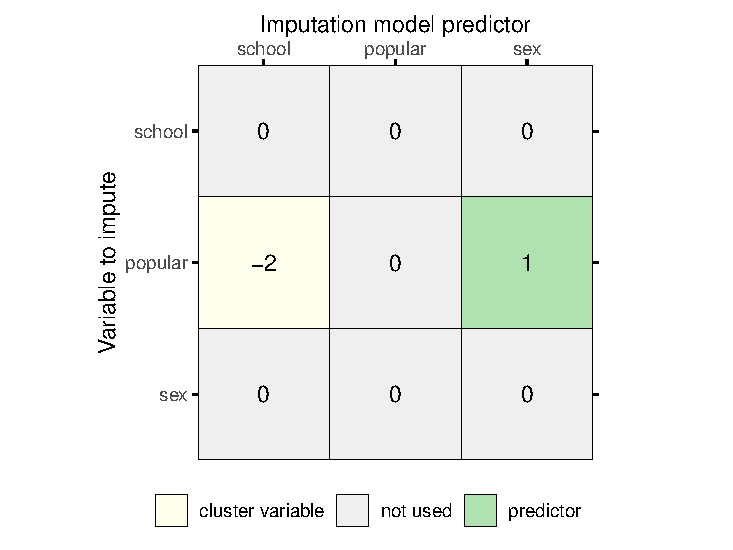
\includegraphics{Imputation_of_Incomplete_Multilevel_Data_files/figure-latex/pop_multilevel-1} \end{center}

\begin{CodeInput}
R> # impute the data, cluster as predictor
R> imp <- mice(popmis, pred = pred, print = FALSE)
\end{CodeInput}
\end{CodeChunk}

Analyze the imputations:

\begin{CodeChunk}
\begin{CodeInput}
R> fit <- with(imp, 
+             lmer(popular ~ 1 + sex + (1 | school))) 
\end{CodeInput}
\end{CodeChunk}

Print the estimates:

\begin{CodeChunk}
\begin{CodeInput}
R> testEstimates(as.mitml.result(fit), extra.pars = TRUE)
\end{CodeInput}
\begin{CodeOutput}

Call:

testEstimates(model = as.mitml.result(fit), extra.pars = TRUE)

Final parameter estimates and inferences obtained from 5 imputed data sets.

             Estimate Std.Error   t.value        df   P(>|t|)       RIV       FMI 
(Intercept)     5.011     0.410    12.222     4.226     0.000    35.955     0.980 
sex             0.928     0.381     2.434     4.168     0.069    48.221     0.985 

                            Estimate 
Intercept~~Intercept|school    0.313 
Residual~~Residual             1.428 
ICC|school                     0.188 

Unadjusted hypothesis test as appropriate in larger samples.
\end{CodeOutput}
\end{CodeChunk}

\hypertarget{case-study-ii-impact-data-syst-missingness-pred-matrix}{%
\section{Case study II: IMPACT data (syst missingness, pred
matrix)}\label{case-study-ii-impact-data-syst-missingness-pred-matrix}}

We illustrate how to impute incomplete multilevel data by means of a
case study: \texttt{impact} from the \pkg{metamisc} package
\citep[empirical data on traumatic brain injuries, \(n = 11,022\) units
across \(N = 15\) clusters,][]{metamisc}. The \texttt{impact} data set
contains traumatic brain injury data on \(n = 11022\) patients clustered
in \(N = 15\) studies with the following 11 variables:

\begin{itemize}
\tightlist
\item
  \texttt{name} Name of the study,
\item
  \texttt{type} Type of study (RCT: randomized controlled trial, OBS:
  observational cohort),
\item
  \texttt{age} Age of the patient,
\item
  \texttt{motor\_score} Glasgow Coma Scale motor score,
\item
  \texttt{pupil} Pupillary reactivity,
\item
  \texttt{ct} Marshall Computerized Tomography classification,
\item
  \texttt{hypox} Hypoxia (0=no, 1=yes),
\item
  \texttt{hypots} Hypotension (0=no, 1=yes),
\item
  \texttt{tsah} Traumatic subarachnoid hemorrhage (0=no, 1=yes),
\item
  \texttt{edh} Epidural hematoma (0=no, 1=yes),
\item
  \texttt{mort} 6-month mortality (0=alive, 1=dead).
\end{itemize}

The analysis model for this dataset is a prediction model with
\texttt{mort} as the outcome. In this tutorial we'll estimate the
adjusted prognostic effect of \texttt{ct} on mortality outcomes. The
estimand is the adjusted odds ratio for \texttt{ct}, after including
\texttt{type}, \texttt{age} \texttt{motor\_score} and \texttt{pupil}
into the analysis model:

\begin{CodeChunk}
\begin{CodeInput}
R> mod <- mort ~ 1 + type + age + motor_score + pupil + ct + (1 | name) 
\end{CodeInput}
\end{CodeChunk}

Note that variables \texttt{hypots}, \texttt{hypox}, \texttt{tsah} and
\texttt{edh} are not part of the analysis model, and may thus serve as
auxiliary variables for imputation.

The \texttt{impact} data included in the \pkg{metamisc} package is a
complete data set. The original data has already been imputed once
(Steyerberg et al, 2008). For the purpose of this tutorial we have
induced missingness (mimicking the missing data in the original data set
before imputation). The resulting incomplete data can be accessed from
\href{https://zenodo.com}{zenodo link to be created}.

Load the complete and incomplete data into the R workspace:

\begin{CodeChunk}
\begin{CodeInput}
R> data("impact", package = "metamisc")      # complete data
R> dat <- read.table("link/to/the/data.txt") # incomplete data
\end{CodeInput}
\end{CodeChunk}

The estimated effects in the complete data are visualized in Figure
\ref{}.

\begin{CodeChunk}


\begin{center}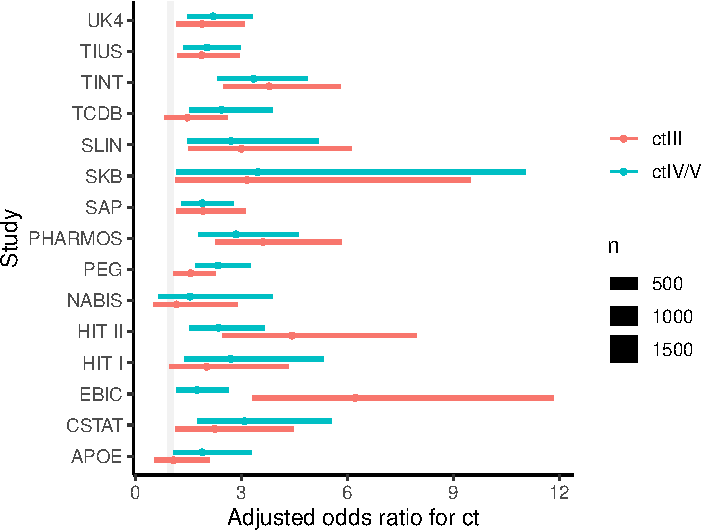
\includegraphics{Imputation_of_Incomplete_Multilevel_Data_files/figure-latex/forest-1} \end{center}

\end{CodeChunk}

\begin{CodeChunk}
\begin{CodeInput}
R> # fit <- glmer(mod, family = "binomial", data = impact) # fit the model
R> # tidy(fit, conf.int = TRUE, exponentiate = TRUE)       # print estimates
\end{CodeInput}
\end{CodeChunk}

\hypertarget{missingness}{%
\subsection{Missingness}\label{missingness}}

To explore the missingness, it is wise to look at the missing data
pattern. The ten most frequent missingness patterns are shown:

\begin{CodeChunk}
\begin{CodeInput}
R> plot_pattern(dat, rotate = TRUE)  # plot missingness pattern
\end{CodeInput}


\begin{center}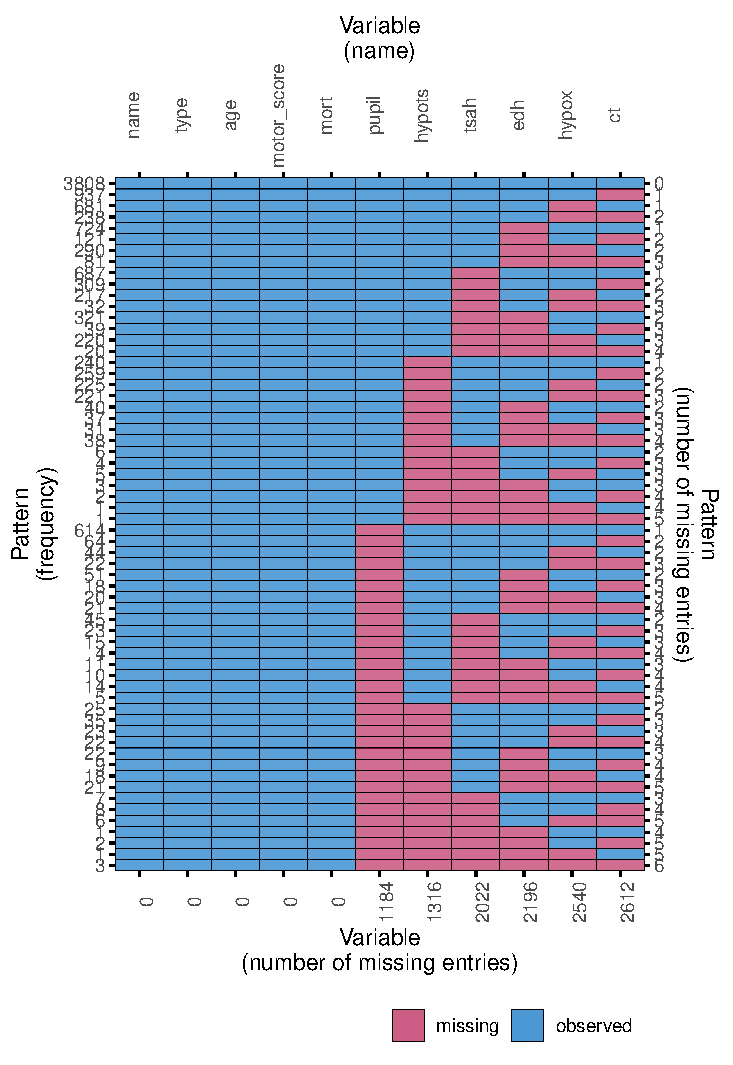
\includegraphics{Imputation_of_Incomplete_Multilevel_Data_files/figure-latex/pattern-1} \end{center}

\end{CodeChunk}

This shows that we need to impute \texttt{ct} and \texttt{pupil}.

To develop the best imputation model, we need to investigate the
relations between the observed values of the incomplete variables and
the observed values of other variables, and the relation between the
missingness indicators of the incomplete variables and the observed
values of the other variables. To see whether the missingness depends on
the observed values of other variables, we can test this statistically
or use visual inspection (e.g.~a histogram faceted by the missingness
indicator).

We should impute the variables \texttt{ct} and \texttt{pupil} and any
auxiliary variables we might want to use to impute these incomplete
analysis model variables. We can evaluate which variables may be useful
auxiliaries by plotting the pairwise complete correlations:

\begin{CodeChunk}
\begin{CodeInput}
R> plot_corr(dat, rotate = TRUE) # plot correlations 
\end{CodeInput}


\begin{center}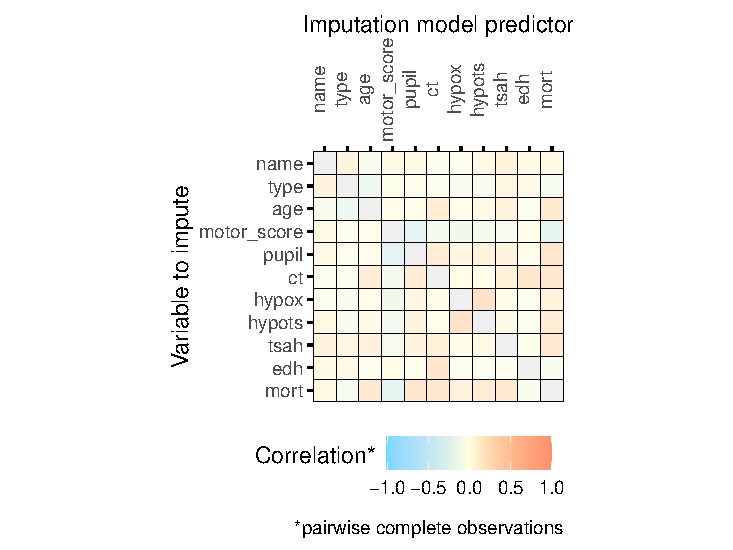
\includegraphics{Imputation_of_Incomplete_Multilevel_Data_files/figure-latex/impact_corr-1} \end{center}

\end{CodeChunk}

This shows us that \texttt{hypox} and \texttt{hypot} would not be useful
auxiliary variables for imputing \texttt{ct}. Depending on the minimum
required correlation, \texttt{tsah} could be useful, while \texttt{edh}
has the strongest correlation with \texttt{ct} out of all the variables
in the data and should definitely be included in the imputation model.
For the imputation of \texttt{pupil}, none of the potential auxiliary
variables has a very strong relation, but \texttt{hypots} could be used.
We conclude that we can exclude \texttt{hypox} from the data, since this
is neither an analysis model variable nor an auxiliary variable for
imputation:

\begin{CodeChunk}
\begin{CodeInput}
R> dat <- select(dat, !hypox)  # remove variable
\end{CodeInput}
\end{CodeChunk}

\hypertarget{complete-case-analysis}{%
\subsection{Complete case analysis}\label{complete-case-analysis}}

As previously stated, complete case analysis lowers statistical power
and may bias results. The complete case analysis estimates are:

\begin{CodeChunk}
\begin{CodeInput}
R> fit <- glmer(mod, family = "binomial", data = na.omit(dat)) # fit the model
R> tidy(fit, conf.int = TRUE, exponentiate = TRUE)             # print estimates
\end{CodeInput}
\begin{CodeOutput}
# A tibble: 11 x 9
   effect  group term  estimate std.error statistic   p.value conf.low conf.high
   <chr>   <chr> <chr>    <dbl>     <dbl>     <dbl>     <dbl>    <dbl>     <dbl>
 1 fixed   <NA>  (Int~   0.0863   0.0182     -11.6   3.00e-31   0.0571     0.130
 2 fixed   <NA>  type~   0.757    0.137       -1.54  1.22e- 1   0.531      1.08 
 3 fixed   <NA>  age     1.03     0.00265     12.9   7.40e-38   1.03       1.04 
 4 fixed   <NA>  moto~   0.651    0.0732      -3.82  1.34e- 4   0.522      0.811
 5 fixed   <NA>  moto~   0.489    0.0555      -6.30  2.97e-10   0.391      0.611
 6 fixed   <NA>  moto~   0.274    0.0321     -11.0   2.28e-28   0.218      0.345
 7 fixed   <NA>  pupi~   3.20     0.317       11.7   8.18e-32   2.63       3.88 
 8 fixed   <NA>  pupi~   1.75     0.195        5.06  4.27e- 7   1.41       2.18 
 9 fixed   <NA>  ctIII   2.41     0.268        7.89  3.05e-15   1.94       2.99 
10 fixed   <NA>  ctIV~   2.30     0.214        8.95  3.56e-19   1.92       2.76 
11 ran_pa~ name  sd__~   0.230   NA           NA    NA         NA         NA    
\end{CodeOutput}
\end{CodeChunk}

As we can see, a higher \texttt{ct} (Marshall Computerized Tomography
classification) is associated with a lower odds of 6-month mortality,
given by the odds ratio exp(0.42), CI \ldots{} to \ldots, when
controlling for\ldots{}

\hypertarget{imputation-model}{%
\subsection{Imputation model}\label{imputation-model}}

Mutate data to get the right data types for imputation (e.g.~integer for
clustering variable).

\begin{CodeChunk}
\begin{CodeInput}
R> dat <- dat %>% mutate(across(everything(), as.integer))
\end{CodeInput}
\end{CodeChunk}

Create a methods vector and predictor matrix, and make sure
\texttt{name} is not included as predictor, but as clustering variable:

\begin{CodeChunk}
\begin{CodeInput}
R> meth <- make.method(dat) # methods vector
R> pred <- quickpred(dat)   # predictor matrix
R> plot_pred(pred, rotate = TRUE)
\end{CodeInput}


\begin{center}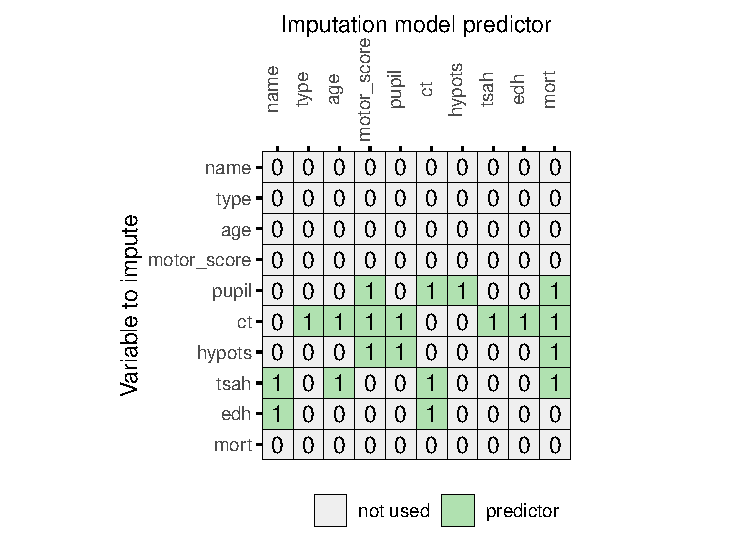
\includegraphics{Imputation_of_Incomplete_Multilevel_Data_files/figure-latex/impact-1} \end{center}

\begin{CodeInput}
R> pred[pred == 1] <- 2
R> pred["mort", ] <- 2
R> pred[, "mort"] <- 2
R> pred[c("name", "type", "age", "motor_score", "mort"), ] <- 0
R> pred[, "name"] <- -2
R> diag(pred) <- 0
R> plot_pred(pred, rotate = TRUE)
\end{CodeInput}


\begin{center}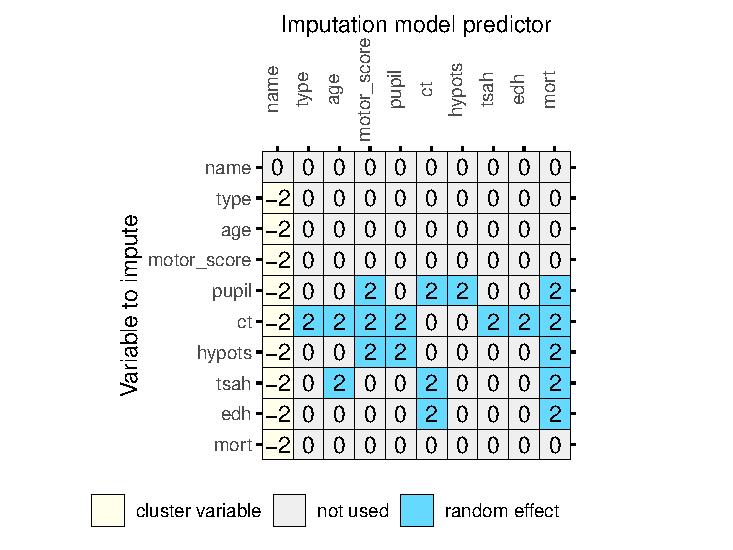
\includegraphics{Imputation_of_Incomplete_Multilevel_Data_files/figure-latex/impact-2} \end{center}

\begin{CodeInput}
R> meth <- make.method(dat)
R> meth
\end{CodeInput}
\begin{CodeOutput}
       name        type         age motor_score       pupil          ct 
         ""          ""          ""          ""       "pmm"       "pmm" 
     hypots        tsah         edh        mort 
      "pmm"       "pmm"       "pmm"          "" 
\end{CodeOutput}
\end{CodeChunk}

Impute the incomplete data

\begin{CodeChunk}
\begin{CodeInput}
R> imp <- mice(dat, method = meth, predictorMatrix = pred, printFlag = FALSE)
\end{CodeInput}
\end{CodeChunk}

\begin{CodeChunk}
\begin{CodeInput}
R> fit <- imp %>% 
+   with(glmer(mort ~ type + age + as.factor(motor_score) + pupil + ct + (1 | name), family = "binomial")) 
R> tidy(pool(fit))
\end{CodeInput}
\begin{CodeOutput}
                     term    estimate   std.error  statistic      p.value
1             (Intercept) -2.35203726 0.340181747  -6.914061 4.994037e-12
2                    type -0.41265892 0.180274846  -2.289054 2.209524e-02
3                     age  0.03049023 0.001570162  19.418521 1.238416e-81
4 as.factor(motor_score)2 -0.66764920 0.068737865  -9.712975 3.480413e-22
5 as.factor(motor_score)3 -1.05520001 0.070218940 -15.027285 2.540225e-50
6 as.factor(motor_score)4 -1.51238349 0.072304262 -20.916934 1.850073e-90
7                   pupil  0.48421447 0.038982800  12.421234 6.772069e-17
8                      ct  0.43474621 0.029968474  14.506785 2.342253e-36
             b          df dfcom         fmi      lambda m         riv
1 5.281599e-04 10119.70041 11013 0.005673265 0.005476771 5 0.005506932
2 4.881699e-05 10893.89378 11013 0.001985736 0.001802528 5 0.001805783
3 3.335358e-08  6320.89582 11013 0.016545467 0.016234340 5 0.016502243
4 4.188703e-05  8327.24771 11013 0.010875748 0.010638213 5 0.010752602
5 5.135721e-05  7632.20045 11013 0.012757637 0.012498967 5 0.012657168
6 1.403058e-04  2831.75462 11013 0.032888241 0.032205434 5 0.033277139
7 3.571497e-04    49.97295 11013 0.309130930 0.282023647 5 0.392803531
8 8.586645e-05   294.69765 11013 0.120677044 0.114729598 5 0.129598366
          ubar
1 1.150898e-01
2 3.244044e-02
3 2.425385e-06
4 4.674630e-03
5 4.869071e-03
6 5.059539e-03
7 1.091079e-03
8 7.950697e-04
\end{CodeOutput}
\begin{CodeInput}
R> as.mitml.result(fit)
\end{CodeInput}
\begin{CodeOutput}
[[1]]
Generalized linear mixed model fit by maximum likelihood (Laplace
  Approximation) [glmerMod]
 Family: binomial  ( logit )
Formula: mort ~ type + age + as.factor(motor_score) + pupil + ct + (1 |  
    name)
      AIC       BIC    logLik  deviance  df.resid 
10495.423 10561.192 -5238.712 10477.423     11013 
Random effects:
 Groups Name        Std.Dev.
 name   (Intercept) 0.2843  
Number of obs: 11022, groups:  name, 15
Fixed Effects:
            (Intercept)                     type                      age  
               -2.37195                 -0.41014                  0.03052  
as.factor(motor_score)2  as.factor(motor_score)3  as.factor(motor_score)4  
               -0.65802                 -1.04611                 -1.51245  
                  pupil                       ct  
                0.50405                  0.42496  
optimizer (Nelder_Mead) convergence code: 0 (OK) ; 0 optimizer warnings; 1 lme4 warnings 

[[2]]
Generalized linear mixed model fit by maximum likelihood (Laplace
  Approximation) [glmerMod]
 Family: binomial  ( logit )
Formula: mort ~ type + age + as.factor(motor_score) + pupil + ct + (1 |  
    name)
     AIC      BIC   logLik deviance df.resid 
10500.88 10566.65 -5241.44 10482.88    11013 
Random effects:
 Groups Name        Std.Dev.
 name   (Intercept) 0.2917  
Number of obs: 11022, groups:  name, 15
Fixed Effects:
            (Intercept)                     type                      age  
               -2.37718                 -0.41511                  0.03067  
as.factor(motor_score)2  as.factor(motor_score)3  as.factor(motor_score)4  
               -0.66935                 -1.05211                 -1.49429  
                  pupil                       ct  
                0.49013                  0.43835  
optimizer (Nelder_Mead) convergence code: 0 (OK) ; 0 optimizer warnings; 1 lme4 warnings 

[[3]]
Generalized linear mixed model fit by maximum likelihood (Laplace
  Approximation) [glmerMod]
 Family: binomial  ( logit )
Formula: mort ~ type + age + as.factor(motor_score) + pupil + ct + (1 |  
    name)
      AIC       BIC    logLik  deviance  df.resid 
10505.026 10570.795 -5243.513 10487.026     11013 
Random effects:
 Groups Name        Std.Dev.
 name   (Intercept) 0.2908  
Number of obs: 11022, groups:  name, 15
Fixed Effects:
            (Intercept)                     type                      age  
               -2.32339                 -0.42359                  0.03023  
as.factor(motor_score)2  as.factor(motor_score)3  as.factor(motor_score)4  
               -0.67142                 -1.05776                 -1.51038  
                  pupil                       ct  
                0.49756                  0.42474  
optimizer (Nelder_Mead) convergence code: 0 (OK) ; 0 optimizer warnings; 1 lme4 warnings 

[[4]]
Generalized linear mixed model fit by maximum likelihood (Laplace
  Approximation) [glmerMod]
 Family: binomial  ( logit )
Formula: mort ~ type + age + as.factor(motor_score) + pupil + ct + (1 |  
    name)
      AIC       BIC    logLik  deviance  df.resid 
10519.511 10585.280 -5250.755 10501.511     11013 
Random effects:
 Groups Name        Std.Dev.
 name   (Intercept) 0.2961  
Number of obs: 11022, groups:  name, 15
Fixed Effects:
            (Intercept)                     type                      age  
               -2.33581                 -0.40871                  0.03039  
as.factor(motor_score)2  as.factor(motor_score)3  as.factor(motor_score)4  
               -0.66477                 -1.05451                 -1.51858  
                  pupil                       ct  
                0.45928                  0.44419  
optimizer (Nelder_Mead) convergence code: 0 (OK) ; 0 optimizer warnings; 2 lme4 warnings 

[[5]]
Generalized linear mixed model fit by maximum likelihood (Laplace
  Approximation) [glmerMod]
 Family: binomial  ( logit )
Formula: mort ~ type + age + as.factor(motor_score) + pupil + ct + (1 |  
    name)
      AIC       BIC    logLik  deviance  df.resid 
10522.038 10587.807 -5252.019 10504.038     11013 
Random effects:
 Groups Name        Std.Dev.
 name   (Intercept) 0.2955  
Number of obs: 11022, groups:  name, 15
Fixed Effects:
            (Intercept)                     type                      age  
               -2.35187                 -0.40574                  0.03064  
as.factor(motor_score)2  as.factor(motor_score)3  as.factor(motor_score)4  
               -0.67468                 -1.06551                 -1.52622  
                  pupil                       ct  
                0.47006                  0.44148  
optimizer (Nelder_Mead) convergence code: 0 (OK) ; 0 optimizer warnings; 1 lme4 warnings 

attr(,"class")
[1] "mitml.result" "list"        
\end{CodeOutput}
\begin{CodeInput}
R> # testEstimates(as.mitml.result(fit))
\end{CodeInput}
\end{CodeChunk}

\hypertarget{case-study-iii-obesity-data}{%
\section{Case study III: obesity
data}\label{case-study-iii-obesity-data}}

In this example, we demonstrate a multilevel imputation of an intercept
and slope random model with a continuous response. We use the obesity
dataset included in the \texttt{micemd}@ package, a synthetic dataset
that emulates an electronic survey in which individuals are asked to
provide information about their weight and consumption habits in
different countries. To easy the explanations we simulate data for 5
clusters and we reduce the dataset to the following variables:

\begin{itemize}
\tightlist
\item
  \texttt{region} Cluster variable,
\item
  \texttt{gender} Gender (0=male, 1=female),
\item
  \texttt{age} Age of the patient,
\item
  \texttt{height} Height in meters,
\item
  \texttt{weight} Weight in kilograms,
\item
  `time`` Response time in minutes (inclusion-restriction variable).
\item
  `FamOb`` Family obesity history (yes or not)
\end{itemize}

In this dataset, Age and FamOb are MAR, while the weight variable is
affected by selection bias, attributed to an indirect MNAR mechanism.
This MNAR mechanism typically arises when an unobserved or omitted
variable influences both the value of the incomplete variable (in this
case, Weight) and its likelihood of being missing (denoted as R).

In the primary analysis model, BMI serves as the dependent variable,
with Age, Gender, and FamOb as predictors. Researchers, based on
observable data, are considering the inclusion of random intercept
effects, as well as introducing a random slope for the Age variable.

The main model is given by:
\[BMI_{ij}= (\beta_{o}+ b_{oj} ) + (\beta_{1}+ b_{oj})* Age_{ij} + \beta_{2}*FamOb_{ij}+ \beta_{3}Gender_{ij} + \epsilon_{ij}\]
We start by loading the data:

\begin{CodeChunk}
\begin{CodeInput}
R> #data("data_heckman", package = "micemd")
R> #dat <- data_heckman
\end{CodeInput}
\end{CodeChunk}

Now, let's begin by examining the missing patterns in the data by
cluster:

\begin{CodeChunk}
\begin{CodeInput}
R> require(patchwork)
R>   myplots <- lapply(1:5, function(i) {
+          ggmice::plot_pattern(setDT(Obesity)[Cluster==i])+ 
+          ggplot2::ggtitle(paste0("Cluster", i))+ 
+          ggplot2::theme(legend.position = ifelse(i==1,"bottom","none"))
+       })
R>   myplots[[1]]+ myplots[[2]] /myplots[[3]]+ myplots[[4]] /myplots[[5]]
\end{CodeInput}


\begin{center}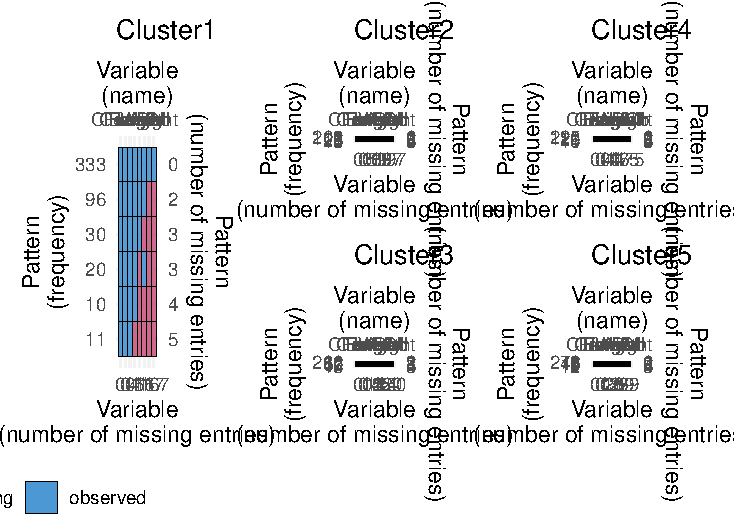
\includegraphics{Imputation_of_Incomplete_Multilevel_Data_files/figure-latex/obesity-md-1} \end{center}

\end{CodeChunk}

We observe that the missing pattern is quite similar across the
clusters. However, regarding the weight variable, we notice that is
systematically missing in cluster 3. In order to evaluate if it is
required a imputation method for 1-level or 2-level we assess the
Intraclass Correlation Coefficient (ICC) for the outcome variable, we
use the ``performance'' package:

\begin{CodeChunk}
\begin{CodeInput}
R> Nulmodel <- lme4::lmer(BMI ~ 1 + (1|Cluster), data = Obesity)
R> performance::icc(Nulmodel)
\end{CodeInput}
\begin{CodeOutput}
# Intraclass Correlation Coefficient

    Adjusted ICC: 0.362
  Unadjusted ICC: 0.362
\end{CodeOutput}
\end{CodeChunk}

Since the ICC is above 0.1 and as the main analyis will be consider a
mixed model, we decide to use two-level (2l) imputation methods. In this
imputation process, we include all predictor variables in the main model
and since BMI is a composite variable. We also incorporate weight and
height variables.

To determine the best imputation method for these variables, we can use
the \texttt{find.defaultMethod}function provided in the \texttt{micemd}
package, which suggests an appropriate method for MAR variables based on
the type of variable, number of observations in the cluster, and number
of clusters. It suggests using ``2l.2stage.bin'' for the FAV variable
and ``2l.2stage.norm'' for the age variable. However, after inspecting
the age density plot, we consider modifying its method to
``2l.2stage.pmm.'' For the BMI variable, we employ deterministic
imputation.

\begin{CodeChunk}
\begin{CodeInput}
R> meth_mar <- meth_mar <- find.defaultMethod(Obesity, ind.clust=1, I.small = 7, ni.small = 100, prop.small = 0.4)
R> meth_mar["BMI"]<- "~ I(Weight / (Height)^2)"
R> meth_mar["Age"]<-"2l.2stage.pmm" 
\end{CodeInput}
\end{CodeChunk}

For these imputation models, it is necessary to specify the prediction
matrix, with the cluster variable labeled as -2 and the predictor
variable labeled as 2, encompassing all variables. We need to suprime
the variable Time as this variable is not especified in the main model
and modify also in the prediction matrix the relationship between BMI,
weight and height to avoid circular predictions. Then we proced to run
the imputation model.

\begin{CodeChunk}
\begin{CodeInput}
R> pred_mar <- mice(Obesity, maxit = 0)$pred   # predictor matrix
R> pred_mar[,"Cluster"]<- -2 # clustering variable
R> pred_mar[,"Time"]<-0
R> pred_mar[pred_mar==1]<-2
R> pred_mar[c("Height", "Weight"), "BMI"] <- 0
R> ggmice::plot_pred(pred_mar)
\end{CodeInput}


\begin{center}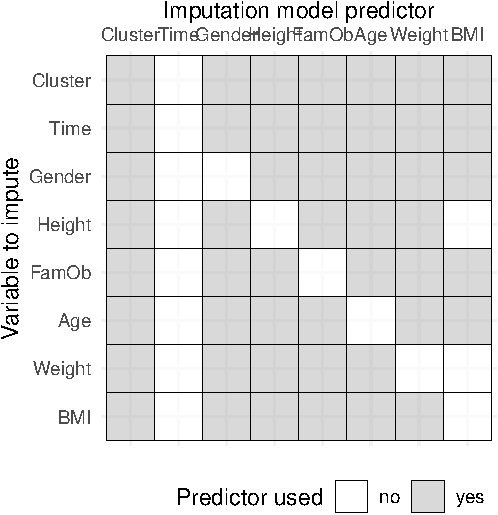
\includegraphics{Imputation_of_Incomplete_Multilevel_Data_files/figure-latex/obsmar_pred-1} \end{center}

\end{CodeChunk}

\begin{CodeChunk}
\begin{CodeInput}
R> summary(complete(imp_mar,"long")$Weight)
\end{CodeInput}
\begin{CodeOutput}
   Min. 1st Qu.  Median    Mean 3rd Qu.    Max. 
 -19.48   68.45   81.65   81.28   94.12  160.76 
\end{CodeOutput}
\begin{CodeInput}
R> plot(imp_mar)
\end{CodeInput}


\begin{center}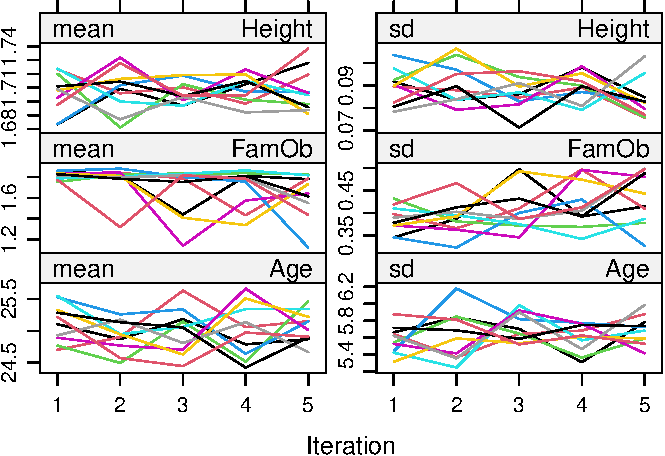
\includegraphics{Imputation_of_Incomplete_Multilevel_Data_files/figure-latex/obsmar_plot-1} \end{center}



\begin{center}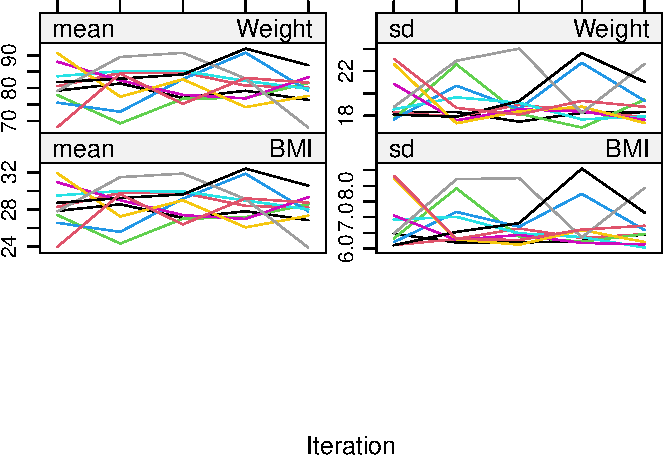
\includegraphics{Imputation_of_Incomplete_Multilevel_Data_files/figure-latex/obsmar_plot-2} \end{center}

\end{CodeChunk}

We are also contemplating the utilization of the ``pmm'' option, given
that the imputed values' weights are lower than those of the observable
values.

\begin{CodeChunk}
\begin{CodeInput}
R> summary(complete(imp_mar_pmm,"long")$Weight)
\end{CodeInput}
\begin{CodeOutput}
   Min. 1st Qu.  Median    Mean 3rd Qu.    Max. 
  28.35   69.55   82.54   82.47   94.83  134.61 
\end{CodeOutput}
\begin{CodeInput}
R> plot(imp_mar_pmm)
\end{CodeInput}


\begin{center}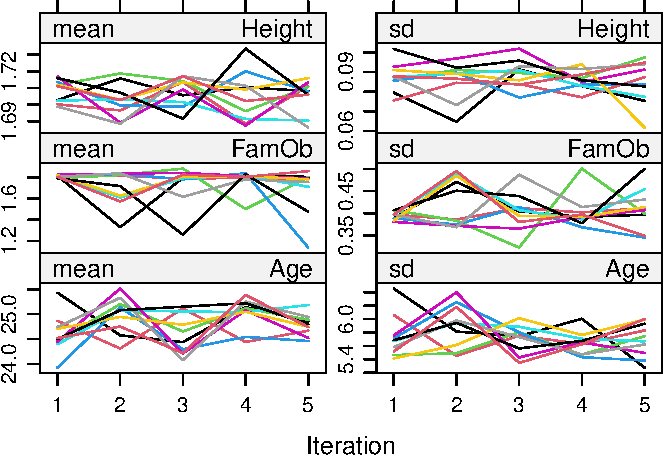
\includegraphics{Imputation_of_Incomplete_Multilevel_Data_files/figure-latex/obsmarp_plot-1} \end{center}



\begin{center}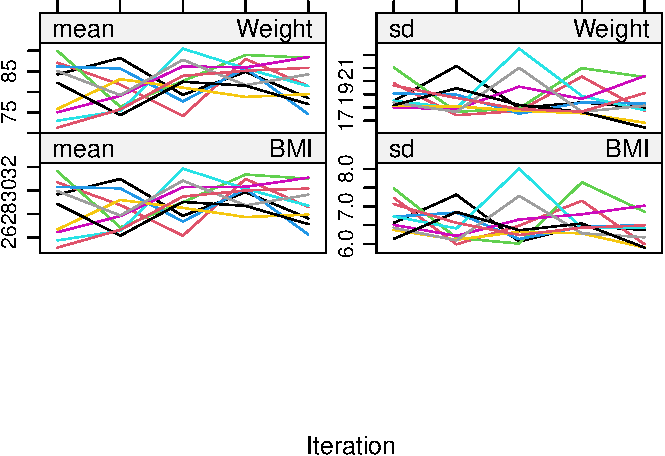
\includegraphics{Imputation_of_Incomplete_Multilevel_Data_files/figure-latex/obsmarp_plot-2} \end{center}

\end{CodeChunk}

After confirming convergence, we proceed to save the results for future
use. Users are considering the possibility that the weight variable may
not have been selected randomly. It's likely that an omitted variable,
like self-esteem, could influence this selection. For instance,
individuals with lower self-esteem might have higher weight values,
impacting their willingness to provide honest information due to
embarrassment.

To address this situation, two approaches have been proposed for dealing
with Missing Not at Random (MNAR) data: pattern-mixed models and
selection models. Within pattern-mixed models, methods like the delta
method and more advanced ones like NARFS have been suggested. In
contrast, the selection model approach includes methods such as the
Heckman model, which can be particularly useful in this case. Several
methods, including Galimar2017, Hammon2021, and the recent Munoz method,
designed for two-level data, allowing for variations in intercepts and
exposure effects (random intercept and slope).

To apply the heckman method, the weight variable should be specified as
``2l.2stage.heckman'' found in the micemd package. Additionally, the
prediction matrix needs modification because this method involves
specifying two equations: one for the outcome, describing the incomplete
variable in terms of partially observed predictors (in this case, all
variables from the main model), and the other for the selection model,
explaining the probability of being observed based (R) on certain
variables.

Here for the outcome equation we consider is the same imputation model
that we used for the MAR case (main model).
\[Weight_{ij}= \beta^O_{o} + \beta^O_{1}* Age_{ij} + \beta^O_{2}*FamOb_{ij}+ \beta^O_{3}Gender_{ij} + \epsilon^O_{ij}\]
Regarding the selection equation, we include the same predictors as
those in the primary model, as well as a time variable. Here the time
variable serves as a restriction exclusion variable specifically
explaining the probability of being observed but not affecting the
incomplete value (Weight). In this context, we assume that the time a
user spends completing the survey serves as a proxy for the barriers
they may encounter in survey completion, such as familiarity with the
survey content or internet speed. These factors may lead the user to
skip specific questions or even the entire survey. Also we assume the
time is not have any influence on the weight assigned to the subject.
\[R_{ij}= \beta^S_{o} + \beta^S_{1}* Age_{ij} + \beta^S_{2}*FamOb_{ij}+ \beta^S_{3}Gender_{ij} +\beta^S_{4}Time_{ij}+ \epsilon^S_{ij}\]
These two equations are jointly estimated under the assumption that the
error terms are interconnected with a bivariate normal distribution. For
a more comprehensive understanding of the model and the exclusion
restriction, you can refer to (Munoz).

To integrate information from both equations, we must adjust the
prediction matrix. The cluster variable remains specified as before
(-2). In this imputation method, all the variables present in both the
selection and outcome equations are included with a random effect.
However, it's essential to distinguish which of these variables appear
in each equation.

In this framework, when a variable is shared between both equations, it
is denoted as (2). Predictors exclusive to the outcome equation are
indicated as (-4), while those exclusive to the selection equation are
labeled as (-3). Consequently, the only alteration needed in the
predictor matrix pertains to the variable ``Time.''

\begin{CodeChunk}
\begin{CodeInput}
R> pred_mnar <- pred_mar
R> pred_mnar["Weight","Time"]<- -3
R> ggmice::plot_pred(pred_mnar)
\end{CodeInput}


\begin{center}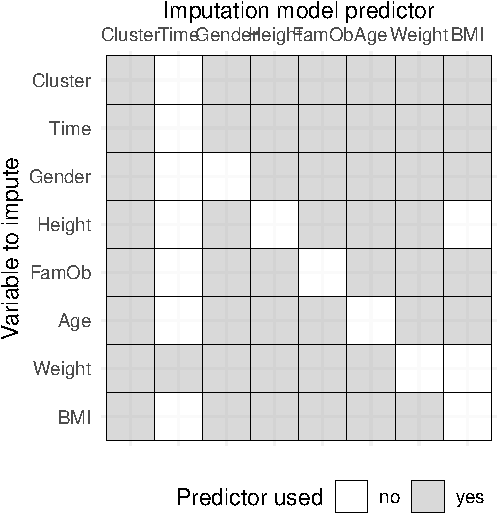
\includegraphics{Imputation_of_Incomplete_Multilevel_Data_files/figure-latex/obsmnar_pred-1} \end{center}

\end{CodeChunk}

We also need to modify the method of the weight variable

\begin{CodeChunk}
\begin{CodeInput}
R> meth_mnar <- meth_mar
R> meth_mnar["Weight"]<- "3l.2stage.heckman"
\end{CodeInput}
\end{CodeChunk}

Then we proceed to run the imputation model as before Impute the
missingness:

After executing these imputation procedures, it is essential to assess
convergence and the coherence of the imputed values. Upon examining the
weight variable, we noticed that the imputed range falls outside the
realm of plausible values (as weight should be positive). Consequently,
we are contemplating a different approach, specifically, the use of
``pmm,'' which involves imputing values from donor observations. This
approach ensures that the imputed values remain within the range of
observable values.

\begin{CodeChunk}
\begin{CodeInput}
R> summary(complete(imp_mnar,"long")$Weight)
\end{CodeInput}
\begin{CodeOutput}
    Min.  1st Qu.   Median     Mean  3rd Qu.     Max. 
 -0.3457  71.4561  84.9177  85.1453  98.5923 182.3955 
\end{CodeOutput}
\begin{CodeInput}
R> plot(imp_mnar)
\end{CodeInput}


\begin{center}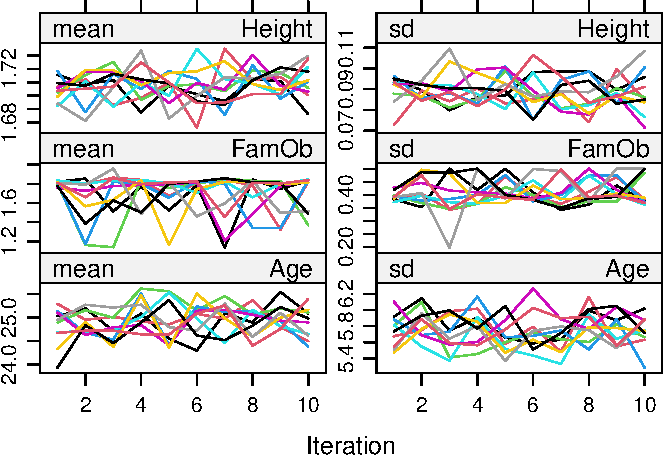
\includegraphics{Imputation_of_Incomplete_Multilevel_Data_files/figure-latex/obsmnar_plot-1} \end{center}



\begin{center}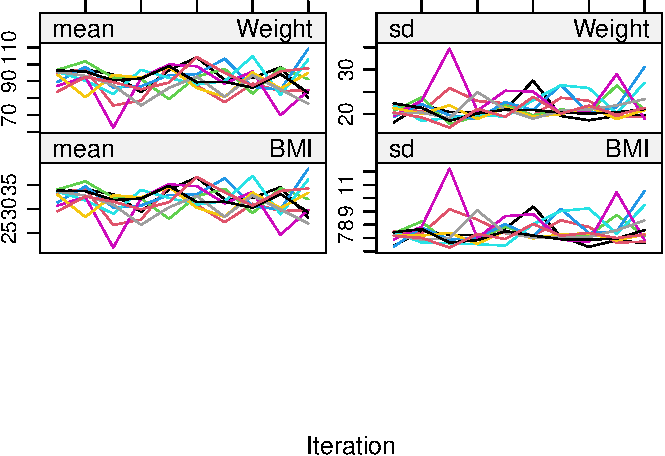
\includegraphics{Imputation_of_Incomplete_Multilevel_Data_files/figure-latex/obsmnar_plot-2} \end{center}

\end{CodeChunk}

We then run the imputation model but this time using the option of pmm,
to assure that weight values are in the range of the observable data,
this can be implemented by seeting the pmm parameter as true.

\begin{CodeChunk}
\begin{CodeInput}
R> summary(complete(imp_mnar_pmm,"long"))
\end{CodeInput}
\begin{CodeOutput}
      .imp           .id          Cluster           Time          Gender     
 Min.   : 1.0   Min.   :   1   Min.   :1.000   Min.   :1.016   Female:10720  
 1st Qu.: 3.0   1st Qu.: 528   1st Qu.:2.000   1st Qu.:3.724   Male  :10390  
 Median : 5.5   Median :1056   Median :3.000   Median :5.151                 
 Mean   : 5.5   Mean   :1056   Mean   :2.868   Mean   :5.211                 
 3rd Qu.: 8.0   3rd Qu.:1584   3rd Qu.:4.000   3rd Qu.:6.698                 
 Max.   :10.0   Max.   :2111   Max.   :5.000   Max.   :9.957                 
     Height      FamOb            Age            Weight            BMI        
 Min.   :1.450   no : 3954   Min.   :14.00   Min.   : 28.35   Min.   : 8.191  
 1st Qu.:1.642   yes:17156   1st Qu.:21.00   1st Qu.: 71.74   1st Qu.:24.699  
 Median :1.701               Median :25.00   Median : 85.36   Median :29.396  
 Mean   :1.702               Mean   :24.88   Mean   : 85.99   Mean   :29.717  
 3rd Qu.:1.761               3rd Qu.:29.00   3rd Qu.: 99.26   3rd Qu.:34.216  
 Max.   :2.012               Max.   :47.00   Max.   :134.61   Max.   :61.911  
\end{CodeOutput}
\begin{CodeInput}
R> plot(imp_mnar_pmm)
\end{CodeInput}


\begin{center}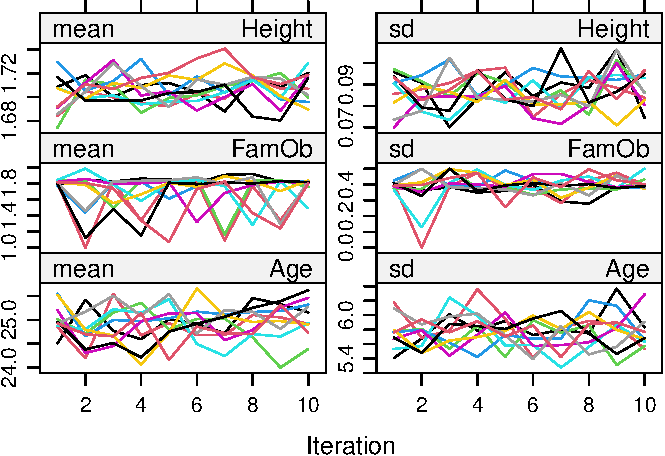
\includegraphics{Imputation_of_Incomplete_Multilevel_Data_files/figure-latex/obsmnarp_plot-1} \end{center}



\begin{center}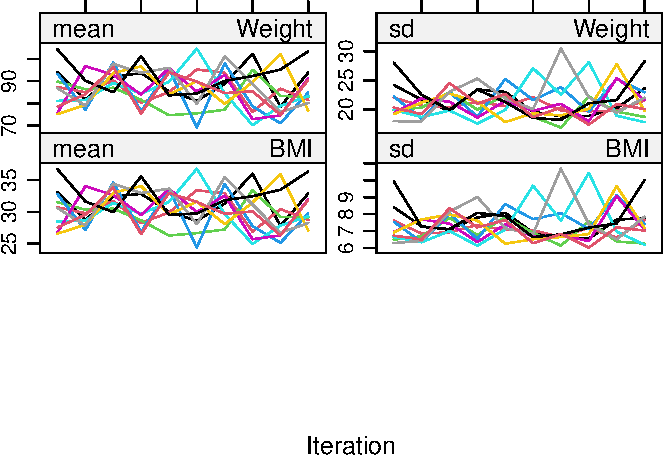
\includegraphics{Imputation_of_Incomplete_Multilevel_Data_files/figure-latex/obsmnarp_plot-2} \end{center}

\end{CodeChunk}

Then after this modification we proceed to compare the effects on the
model, therefore we run the analysis model on each of the completed
datasets along with the dataset where the incomplete values are removed
(CC).

\begin{CodeChunk}
\begin{CodeInput}
R> library(ggplot2)
R> cc_rs<- with(Obesity[complete.cases(Obesity),],lme( BMI ~ Age + FamOb + Gender,random=~1+Age|Cluster))
R> mar_rs <- with(imp_mar,lme( BMI ~ Age + FamOb + Gender,random=~1+Age|Cluster))
R> mar_pmm_rs <- with(imp_mar_pmm,lme( BMI ~ Age + FamOb + Gender,random=~1+Age|Cluster))
R> mnar_rs<- with(imp_mnar,lme(BMI ~ Age + FamOb + Gender,random=~1+Age|Cluster))
R> mnar_pmm_rs<- with(imp_mnar_pmm, lme(BMI ~ Age + FamOb + Gender,random=~1+Age|Cluster))
R> list_models<-list(cc_rs,mar_rs,mar_pmm_rs,mnar_rs,mnar_pmm_rs)
R> plot_models(list_models,mod_name=c("Complete case", "MAR","MAR_pmm", "MNAR", "MNAR_pmm"))
\end{CodeInput}


\begin{center}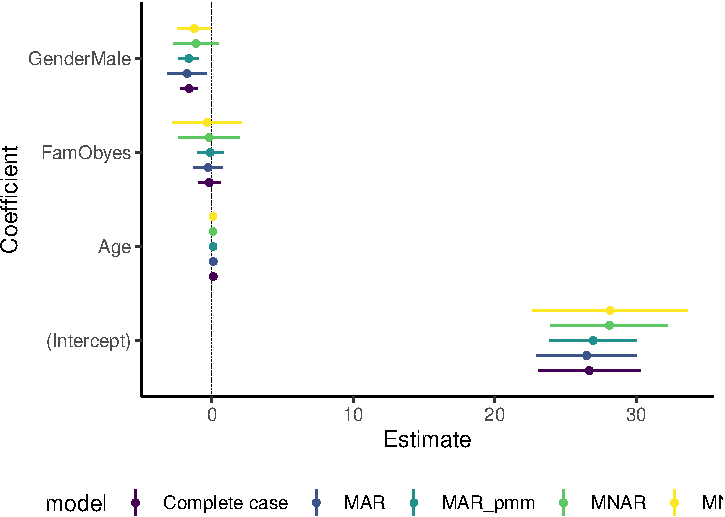
\includegraphics{Imputation_of_Incomplete_Multilevel_Data_files/figure-latex/models-1} \end{center}

\end{CodeChunk}

We note that there is minimal disparity in the age effect, FamObs,
across the various imputation models under consideration. Nonetheless,
with respect to Gender, we observe a notable distinction: in the M(C)AR
assumption, the effect is significant, whereas under the MNAR
assumption, it becomes insignificant. An analysis of the intercept
reveals that, under the MNAR assumption, a higher average BMI is
anticipated compared to the MAR assumption.

Visualize missing data pattern:

The matrix only shows the predictors for the main model, not the
selection model.

\hypertarget{discussion}{%
\section{Discussion}\label{discussion}}

ORDER:

\begin{itemize}
\item
  summary
\item
  congeniality, then in hierarchical models
\item
  look whether we can fit cong. back in the main body
\item
  alt. methods
\item
  conclusion: mice is really easy!
\item
  Additional levels of clustering
\item
  More complex data types: timeseries and polynomial relationship in the
  clustering.
\item
  FIML vs MI
\end{itemize}

An alternative approach to missing data is to use Full Information
Maximum Likelihood (FIML). This method does not require the imputation
of any missing values. Whereas MI consists of imputation, analyses and
pooling steps, FIML analyses the data in a single step. When the
assumptions are met the two approaches should produce equivalent
results. {[}REF{]} As FIML requires specialised software, not all
analyses can be performed with standard software. {[}REF{]}

\begin{itemize}
\tightlist
\item
  Survival / TTE, this could be put in the paragraph on congeniality
\end{itemize}

When the outcome is time-to-event, the Nelson-Aalen estimate of the time
to event should be included as a covariate in the imputation model
{[}REF{]}

In hierarchical datasets, clustering is a concern because the
homoscedasticity in the error terms cannot be assumed across clusters
and the relationship among variables may vary at different hierarchical
levels. When multiple imputation is used to deal with missing data, as
the imputation and analysis process is performed separately, it is
necessary that imputation model being congenial with the main analysis
model (Meng, 1994), e.g.~if the main model accounts for the hierarchical
structure also imputation model should do it (Audigier, 2021). Not
including clustering into the imputation process may lead to effect
estimates with smaller standard errors and inflated type I error.

There are different strategies that can be adopted in the imputation
process that account for clustering: inclusion of cluster indicator
variable, performing a separate imputation process for each cluster, or
performing a simultaneous imputation process by using an imputation
method that accounts for clustering.(Stata:
\url{https://www.stata.com/support/faqs/statistics/clustering-and-mi-impute/})
TODO: replace ref.

The selection of each strategy depends mainly on the assumptions in the
main analysis and also on the restriction of the analyzed data.

Regarding the restrictions imposed by the data, for instance, the use of
cluster indicator variables is restricted in datasets where there are
not many clusters and many observations per cluster (Graham, 2009). The
last restriction is also required when imputations are performed on each
cluster separately. When this restriction cannot be achieved, one can
use an imputation model that simultaneously imputes all clusters using a
hierarchical model (Allison 2002).

Under this hierarchical imputation model, observations within clusters
are correlated and this correlation is modeled by a random effect so the
hierarchical model can be estimated even when there are few observations
per cluster. However, this strategy is best suited for balanced data
(Grund, 2017) and when random effects model is appropriated, i.e.~the
number of clusters is adequate. (Austin,2018).

Here it is important to evaluate the assumptions imposed by the main
model, for instance by using the cluster indicator strategy may lead to
bias estimates when the model is based on a hierarchical model
(Taaljard,2008). Even when an imputation strategy congenial with the
main model is preferred, it is important to consider whether it is
appropriate for the data as a less complex imputation strategies may
also lead to unbiased estimates in certain scenarios(Bailey 2020). For
instance, in causal effect analysis, separately imputation may lead to
smaller bias when the size of the smaller exposure cluster is large,
compared with an imputation model that includes exposure-confounder
interactions. (Zhang,2023).

\hypertarget{funding}{%
\section{Funding}\label{funding}}

This project has received funding from the European Union's Horizon 2020
research and innovation programme under ReCoDID grant agreement No
825746.

The views expressed in this paper are the personal views of the authors
and may not be understood or quoted as being made on behalf of or
reflecting the position of the regulatory agency/agencies or
organizations with which the authors are employed/affiliated.

\hypertarget{references}{%
\section{References}\label{references}}

\hypertarget{appendix}{%
\section{Appendix}\label{appendix}}

Table 3: Notation

\begin{longtable}[]{@{}
  >{\raggedright\arraybackslash}p{(\columnwidth - 2\tabcolsep) * \real{0.5495}}
  >{\raggedright\arraybackslash}p{(\columnwidth - 2\tabcolsep) * \real{0.4505}}@{}}
\toprule\noalign{}
\begin{minipage}[b]{\linewidth}\raggedright
\textbf{Formula \pkg{lme4}}
\end{minipage} & \begin{minipage}[b]{\linewidth}\raggedright
\textbf{Details}
\end{minipage} \\
\midrule\noalign{}
\endhead
\bottomrule\noalign{}
\endlastfoot
\texttt{y\ \textasciitilde{}\ x1\ +\ (1\ \textbar{}\ g1)} & Fixed
\texttt{x1} predictor with random intercept \\
& varying among \texttt{g1} \\
\texttt{y\textasciitilde{}x1*x2+\ (1\textbar{}\ g1)} & Interactions of
\texttt{x1} and \texttt{x2} only in fixed effect \\
\texttt{y\ \textasciitilde{}\ x1*x2+\ (x2\textbar{}\ g1)} & Interactions
of \texttt{x1} and \texttt{x2} only in fixed effect \\
& with slope of \texttt{x2} randomly varying among \texttt{g1} \\
\texttt{y\ \textasciitilde{}\ x1*x2+\ (x1*x2\textbar{}\ g1)} &
variance-covariance matrix estimated only with \\
& the variance terms of intercept, slope of \texttt{x1}, \\
& slope of \texttt{x2} and interaction \texttt{x1*x2} \\
\texttt{y\ \textasciitilde{}\ x1*x2+\ (x1\ \textbar{}\ g1)+\ (x2\textbar{}\ g1)}
& variance-covariance matrix estimated separately, \\
& i.e, one for intercept and \texttt{x1} and another for \\
& intercept and \texttt{x2} \\
\texttt{y\ \textasciitilde{}\ x1\ +\ (x1\ \textbar{}\ g1)\ or\ 1\ +\ x1\ +\ (1\ +\ x1\ \textbar{}\ g1)}
& Fixed \texttt{x1} with correlated random intercept and \\
& random slope of \texttt{x} \\
\texttt{y\ \textasciitilde{}\ x1\ +\ (x1\ \textbar{}\textbar{}\ g1)\ or\ 1\ +\ x1\ +\ (1\ \textbar{}\ g1)\ +\ (0\ +\ x1\ \textbar{}\ g1)}
& Fixed \texttt{x1} with uncorrelated random intercept \\
& and random slope of \texttt{x1} \\
\texttt{y\ \textasciitilde{}\ (1\ \textbar{}\ g1)\ +\ (1\ \textbar{}\ g2)}
& Random intercept varying among \texttt{g1} and among
\texttt{g2\ \ \ \textbar{}\ \textbar{}}y \textasciitilde{} (1 \\
& \\
\end{longtable}

\bibliography{../References/multilevelmice.bib}



\end{document}
